\documentclass[tikz,border=0pt]{standalone}
\usepackage{fontspec,amsmath}
\setmainfont{Arial}
\usetikzlibrary{arrows.meta}
\definecolor{ink}{HTML}{263C4B}
\definecolor{amber}{HTML}{BA8035}
\definecolor{sky}{HTML}{4882B8}
\definecolor{leaf}{HTML}{56895E}
\definecolor{purple}{HTML}{8569A3}
\definecolor{sandbg}{HTML}{FFF3E1}
\definecolor{bluebg}{HTML}{EAF3FC}
\definecolor{greenbg}{HTML}{EDF6E9}
\definecolor{lilacbg}{HTML}{F3EEF9}
\newcommand{\normaltype}{\fontsize{9.5}{11.3}\selectfont}
\newcommand{\headingtype}{\fontsize{11}{12}\selectfont\bfseries}
\begin{document}
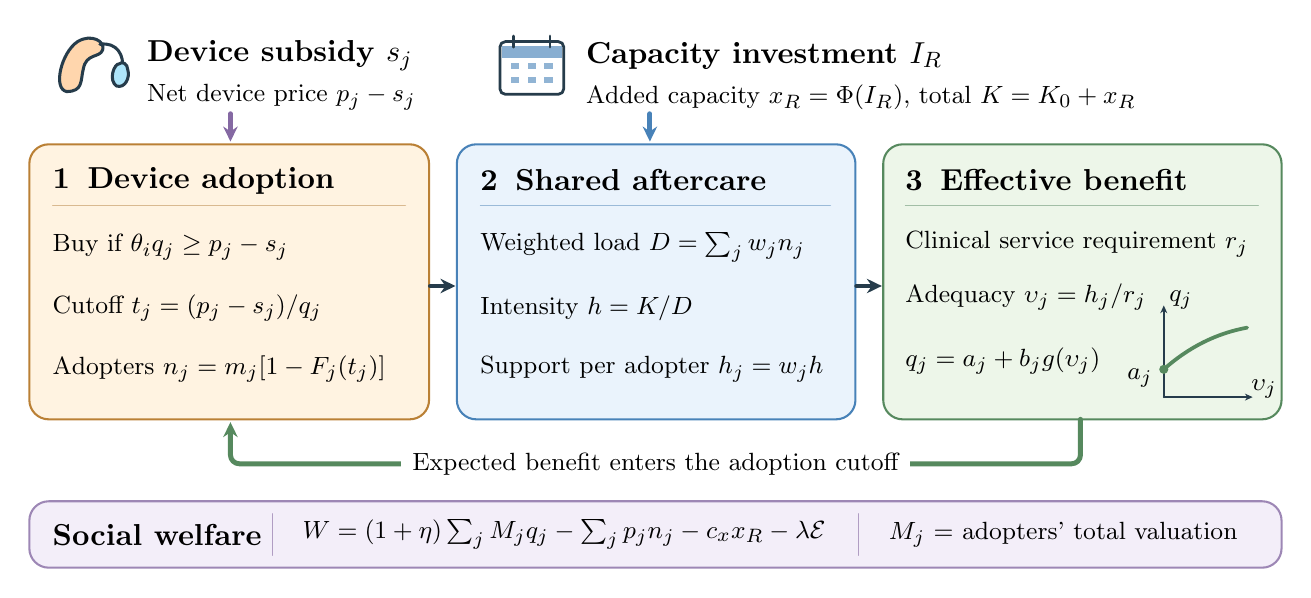
\begin{tikzpicture}[x=1bp,y=1bp,inner sep=0pt,outer sep=0pt,
  font=\normaltype,text=black,line cap=round,line join=round,
  panel/.style={rounded corners=7pt,line width=.75pt},
  link/.style={-{Stealth[length=5.4pt,width=5.2pt]},line width=1.8pt},
  lefttext/.style={anchor=west}]
\path[use as bounding box] (0,0) rectangle (452,195);
% The two policy inputs sit outside the endogenous equilibrium.
\begin{scope}[shift={(9,170)},draw=ink,line width=1.1pt]
  \path[fill=orange!32,draw=ink] (5,2) .. controls (0,3) and (3,16) .. (9,20)
     .. controls (14,23) and (19,20) .. (18,17)
     .. controls (17,14) and (12,16) .. (11,10)
     .. controls (10,6) and (11,2) .. (5,2) -- cycle;
  \draw (17,19) .. controls (23,20) and (26,15) .. (25,10);
  \path[fill=cyan!32,draw=ink] (24,12) .. controls (22,12) and (20,6) .. (23,4)
     .. controls (26,3) and (28,7) .. (27,10) .. controls (27,12) and (25,13) .. (24,12) -- cycle;
\end{scope}
\node[lefttext,font=\headingtype] at (43,185) {Device subsidy $s_j$};
\node[lefttext] at (43,170) {Net device price $p_j-s_j$};
\begin{scope}[shift={(170,170)},draw=ink,line width=1pt]
  \draw[fill=white,rounded corners=2pt] (0,1) rectangle (23,20);
  \fill[sky!65] (.6,14) rectangle (22.4,18.5);
  \draw (5,18)--(5,22) (18,18)--(18,22);
  \foreach \x in {4,10,16} {\foreach \y in {5,10}{\fill[sky!60] (\x,\y) rectangle ++(3,2.4);}}
\end{scope}
\node[lefttext,font=\headingtype] at (201,185) {Capacity investment $I_R$};
\node[lefttext] at (201,170) {Added capacity $x_R=\Phi(I_R)$, total $K=K_0+x_R$};
\draw[link,purple] (73,164)--(73,154);
\draw[link,sky] (224,164)--(224,154);

\draw[panel,draw=amber,fill=sandbg] (.6,54) rectangle (144.5,153);
\draw[panel,draw=sky,fill=bluebg] (154.5,54) rectangle (298,153);
\draw[panel,draw=leaf,fill=greenbg] (308,54) rectangle (451.4,153);
\node[lefttext,font=\headingtype] at (9,140) {1\enspace Device adoption};
\node[lefttext,font=\headingtype] at (163,140) {2\enspace Shared aftercare};
\node[lefttext,font=\headingtype] at (316,140) {3\enspace Effective benefit};
\draw[amber!55] (9,131)--(136,131);
\draw[sky!55] (163,131)--(289,131);
\draw[leaf!55] (316,131)--(443,131);
\node[lefttext] at (9,116) {Buy if $\theta_i q_j\geq p_j-s_j$};
\node[lefttext] at (9,94) {Cutoff $t_j=(p_j-s_j)/q_j$};
\node[lefttext] at (9,72) {Adopters $n_j=m_j[1-F_j(t_j)]$};
\node[lefttext] at (163,116) {Weighted load $D=\sum_j w_jn_j$};
\node[lefttext] at (163,94) {Intensity $h=K/D$};
\node[lefttext] at (163,72) {Support per adopter $h_j=w_jh$};
\node[lefttext] at (316,117) {Clinical service requirement $r_j$};
\node[lefttext] at (316,98) {Adequacy $\upsilon_j=h_j/r_j$};
\node[lefttext] at (316,75) {$q_j=a_j+b_jg(\upsilon_j)$};
% The curve is illustrative; its intercept is positive and its terminal slope is positive.
\draw[-{Stealth[length=2.8pt,width=2.5pt]},ink,line width=.65pt] (409,62)--(409,95);
\draw[-{Stealth[length=2.8pt,width=2.5pt]},ink,line width=.65pt] (409,62)--(441,62);
\draw[leaf,line width=1.35pt] (409,72) .. controls (418,80) and (428,85) .. (439,87);
\fill[leaf] (409,72) circle (1.65pt);
\node[anchor=east] at (405,69) {$a_j$};
\node[anchor=west] at (411,97) {$q_j$};
\node[anchor=west] at (440.5,65) {$\upsilon_j$};
\draw[link,ink] (145,102)--(154,102);
\draw[link,ink] (298.5,102)--(307.5,102);

\draw[link,leaf,rounded corners=3.2pt] (379,54)--(379,38)--(73,38)--(73,53);
\node[fill=white,inner xsep=4pt] at (226,38) {Expected benefit enters the adoption cutoff};
\draw[panel,draw=purple!80,fill=lilacbg] (.6,.6) rectangle (451.4,24.5);
\node[lefttext,font=\headingtype] at (9,12.5) {Social welfare};
\draw[purple!65] (88,5)--(88,20);
\node[lefttext] at (99,12.5)
 {$W=(1+\eta)\sum_j M_jq_j-\sum_j p_jn_j-c_xx_R-\lambda\mathcal E$};
\draw[purple!65] (299,5)--(299,20);
\node[lefttext] at (310,12.5) {$M_j$ = adopters' total valuation};
\end{tikzpicture}
\end{document}
